% !TeX root = ams_thesis.tex
\chapter{UI Design and Implementation}

In order to convert the user gestures collected in the gesture collection experiment into a user interface, a subset of the gestures was selected to support the majority of the user-defined gestures. 

In some cases, the user defined gestures were ambiguous, either across users, or with a user across tasks. 
Where design decisions were made to work around these ambiguities, they are described. 

\section{Selection of Gestures for Control of Swarms}

\begin{figure}
	\centering
	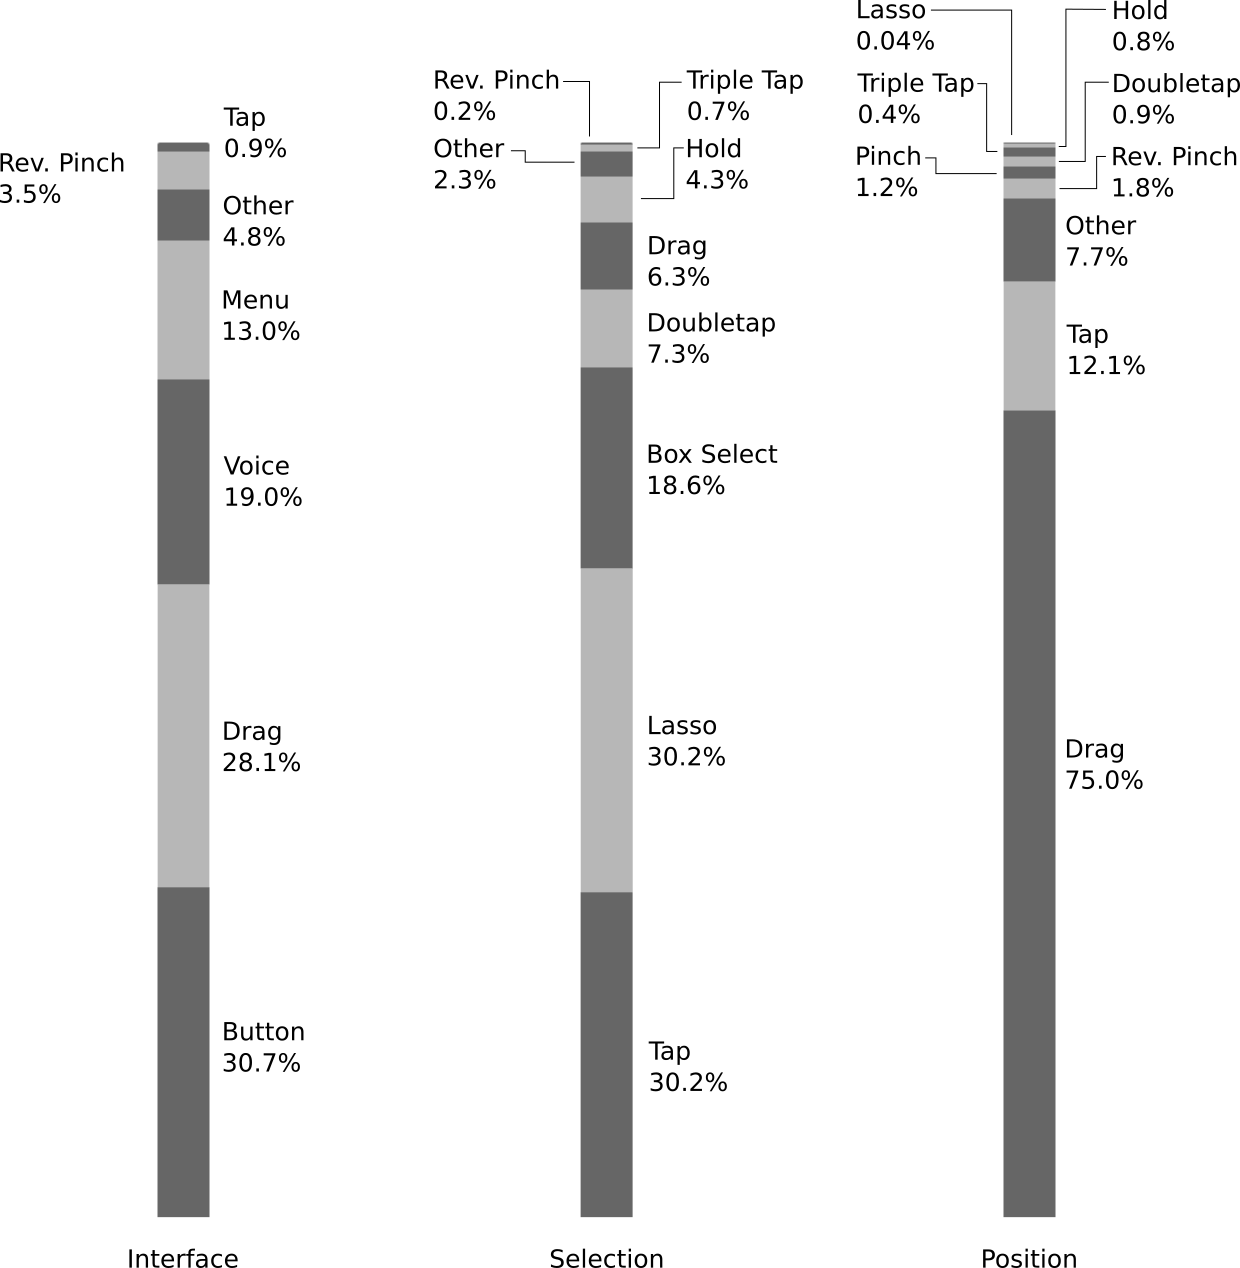
\includegraphics[width=\linewidth]{../thin_grey_text.png}
	\caption{Motion, selection, and UI gestures.}
	\label{fig:select_ui_move_breakdown}
\end{figure}

For position commands, drag, tap, and ``other'' would cover 94.8\% of the gestures. 
Unfortunately, the ``other'' commands are not a single gesture, but include a diverse collection of gestures, such as pushing with the side of the finger or making a picking-up, carrying, and setting-down motion over the screen.
As a consequence, attempting to implement all the gestures in the ``other'' category would add significant complexity to the gesture recognition in order to support gestures that were rarely used. 
Many of the ``other'' gestures were also not recognizable by a multitouch surface, such as the user dividing the robots by parting their hands as if opening a bag in the air above the surface. 
Since it does not contact the multitouch surface, such a gesture cannot be recognized without additional hardware. 
If all forms of tap are considered the same when used as position commands, taps make up 14.2\% of the position commands, and together with drag, cover 89.2\% of the position commands. 

Lasso was used as a position command by one user, who used it to command the robots to disperse in the ``disperse'' task. 
The user noted that the direction of the lasso disambiguated it from lasso as selection, so lassoing clockwise would select robots and lassoing counterclockwise would disperse them. 

Achieving 90\% recognition of the most common UI widgets would include buttons for special functions, handwriting recognition, voice commands, and other menus on the screen (totaling 90.8\%). 
However, a successful menu-based UI would not be composed simply by taking the sum of all of the user interface designs suggested by users, as there would be significant redundancy in the UI commands, and in ways of bringing up the UI for interaction. 
Instead, the tasks that the users invoked the UI in most often were examined, and the requested UI functions were considered for inclusion.

Both voice commands and handwritten commands together account for 47.1\% of the user interface elements used.
While the broad categories make up nearly half of the UI elements, the individual uses of the gestures did not display a significant unity within the broad categories.
One user used symbols drawn over the swarm as commands, so a circle drawn within the swarm area meant ``patrol", and would be followed by an indication of the area to be patrolled. 
Another user wrote commands, such as writing out ``0.5" to indicate that robots should divide in half, ``SQ'' to indicate that they should form a square, or ``C $\rightarrow$ A" to indicate that the crate (C) should be moved to area A. 
The majority of the drawn commands were attributable to a single user, but two users drew an `X' over the defective robot in the ``mark defective robot'' and ``remove defective robot'' tasks and two users used an `X' and an `S' in the ``stop the robots'' task.

The selection of a set of handwritten commands that would be usable for a majority of users would be a task at least as difficult as finding a user-defined set of gestures.
In addition to the set of English letters, the interface would have to consider symbols such as arrows, and apparently decimal numbers as well. 
The experiment described in this thesis did not collect sufficient examples of handwritten commands to extrapolate a useful control scheme from them.
Because of this lack of information, and the fact that most handwritten commands were proposed by a single user, the resulting interface does not contain support for handwriting recognition and symbol interpretation.  

Interestingly, voice commands were similar to both handwriting, in terms of distribution of user choice, and gestures, in terms of syntax. 
One user used voice commands for all tasks, but ten users also used voice commands for at least once. 
The distribution of voice commands is like the handwritten commands, in that one user used handwritten commands frequently, but a few other users used a few of them for some tasks.
The accidental biasing of users towards use of voice for formation tasks was discussed earlier. 
In addition, two users stated that they would like to have a vocal stop command for the ``stop the robots'' task, because it could be issued quickly and without having to accurately touch the moving robots. 
These users did not issue other voice commands, as the other tasks were not perceived to be as urgent as the ``stop the robots'' task. 

\begin{table}
	\centering
	\begin{tabular}{l l}
		Task & Uses of Voice Commands\\
		\hline
		line & 5\\
		square & 4 \\
		crate dispersed & 3 \\
		divide color mix & 3\\
		stop & 3\\
		crate & 2\\
		move a & 2\\
		disperse & 2\\
		merge & 2\\
		split & 2\\
		patrol a & 2 \\
		divide & 1 \\
		divide color 1 & 1\\
		divide color 2 & 1\\
		move wall & 1\\
		remove & 1\\
		mark & 1 \\
		patrol screen & 1\\
	\end{tabular}
	\caption{Use of voice commands by task. The use of high numbers of voice commands for the formation tasks, line and square, was likely biased by the text of the instructional slides. }
\end{table}

The syntactic similarity between the voice commands and the gesture commands is because the gesture commands frequently take the subject-verb-object ordering of spoken sentences. 
Some parallelism in the structure of spoken commands and gestures is  unsurprising, as in human-to-human communication, vocal expressions and gestures are theorized to arise from the same internal representations \citep{mcneill1985so}. 
For example, selecting the robot group indicates a subject, and drawing the path indicates the verb (``go this way"). 
Objects are optional or implied, as going to a location does not have a clear object that the robots are instructed to act upon. 
In some cases, the subject is implied as well.
For example, some users would make gestures intended to move the robot group as a whole by simply dragging the path, without selecting the subject first. 
In such a case, the implied subject was all of the robots. 
This sort of implication is more complex than simply assuming that if no robot is selected, all of the robots are the subject. 
Some users divided the robots into two groups by drawing a dividing line, and then dragging two paths, one to one side of the screen and the other to the other side of the screen. 
In this case, the implied subject was the half of the robots on the same side of the dividing line as the drag, but no selection gesture preceded the positioning drag to indicate this. 

%The idea of having a hidden menu that was dragged in from an edge of the screen or came up after some form of invocation, such as tap-and-hold, was rejected because such menus do not admit exploration. \todo{cite something on explorability/discovery of menus}

Reverse pinch was used as an interface command to zoom in or out of the view of the robots. This was done in the ``mark defective robot'' and ``remove defective robot'' tasks. 
The user who made this gesture was in the 1000 robot case, and stated that they wanted to zoom in because the defective robot was a small target and close to other robots. 
There was no explicit zoom or change of viewpoint task, but users expected the functionality when they had to interact with a small target.

To accommodate 90\% of the user gestures for selection, recognition of tap, lasso, box select, doubletap, drag, hold, and ``other'', totaling 91.9\% of the selection gestures.
As discussed above, the ``other'' category is not practical to implement. 
If, instead, all forms of tap are considered the same for purposes of selection, they comprise 42.5\% of the selection gestures, and together with lasso and box select, cover 91.3\% of the selections. 

Drag as a selection gesture refers to the user placing their finger on one robot, and then dragging it from robot to robot, adding each touched robot to the selection. 
It is ambiguous with the position drag, where the user places their finger on a robot and then drags a path for the robot to follow, although the distinction could be made by having a path that intersects multiple robots become a selection, rather than a position command. 
Unfortunately, this attempt at disambiguation would itself become a source of problems if the user attempts to move the entire swarm by placing a finger in the middle of it and dragging to a new location, as it is likely they would intersect more than one robot as their finger leaves the swarm.

\section{Ambiguities in Gesture Commands}

As discussed briefly in the previous section, some combinations of gestures selected by the users were ambiguous. 
This is to be expected, as the users did not know all the tasks in advance, and so might use a gesture in one task that they then felt was better suited to a later task.
The users might also not regard all the tasks as having to use a consistent and unambiguous representation for each gesture, or not remember all the gestures they had previously used. 
However, for automated conversion into programs, it is important that a sequence of gestures have some way to be unambiguously recognized. 

In the line formation tasks, some users selected the robots and then drew a line to indicate the location of the line formation. 
If the line formation started at the same location as the robots, this gesture sequence is the same as the selection and drawing a path sequence that was frequently used to indicate that the robots should move as a group along the path. 
If the line formation started elsewhere, it could be disambiguated, because motion along a path almost always started on or near the selected robots.  
The user drawing a line over a group of robots could be interpreted a number of ways: as a dividing line, as a box selection, as a path for a single robot to follow, as a path for a group of robots to follow, and as the location of a line formation.

Because a number of other, more explicit commands are available for dividing robots into groups, such as moving one group away from the other, the division line interpretation was rejected. 
A line drawn over robots is treated as a box selection, unless it begins on a single robot. 
In that case it is interpreted as a path for that robot to follow. 
For the purposes of this work, beginning ``on'' a robot was defined as the beginning of the line being within 80 pixels of the location of the robot on the screen. 
80 pixels was selected because it is the approximate width of a human finger on the screen used in this work. 
Obviously, this distance will vary with the resolution of the screen, but the mechanism for obtaining the resolution and physical size of attached screens varies with operating systems, and is outside of the scope of this work, aside from noting that this parameter may vary.

Similarly, some users divided the robots into two groups by drawing a line separating the groups.
Typically, this line started outside the group and passed through it, so it could be disambiguated from instructing the robots to move along the line.
Unfortunately, it would be difficult to separate it from drawing a line for the robots to move to in order to create a formation.

To command the robots into a square formation, especially in the dispersed cases, many users simply drew the square formation over the robots.
If a lasso select is also available, some distinction must be made between the lasso select and the square formation when they are both drawn over the robots, as they are both closed forms drawn over the robots.
One possible method is to look for peaks in the distance from each point on the perimeter of the gesture to the centroid of the gesture. 
A square would have four peaks, while a circle would have no obvious peaks. 
However, this sort of recognition means that a square lasso select, or an arbitrarily-shaped lasso select that happens to have four peaks, would get misinterpreted as a formation gesture, while a command to get into a circular formation would be interpreted as a lasso selection. 
It would be preferable to be able to make arbitrary formations, and arbitrarily-shaped lasso selections, and have them be disambiguated by some other method. 
One method that users proposed was to have a ``draw formation" button, which would then cause the next form that the user drew to be treated as the perimeter of the formation. 
Some users also held one finger down at the start of the formation, while tracing the perimeter with the other finger. 
Using a multi-finger gesture has the advantage of not adding UI elements, but is not easily discoverable by a user examining the UI. 

In order to patrol area A or the screen border, users frequently dragged the robots as if issuing a basic motion command. 
Some users indicated that there would have to be an additional signal to the robots to keep moving on the patrol route, once it was assigned, but there was not an agreement as to what that command should be. 
Of the users who indicated a need to convey that the swarm keep patrolling, some repeated the patrol route drag multiple times, others ended the gesture with a tap or triple tap, still others used the direction of the patrol route drag (clockwise or counterclockwise) to separate following the path once from continuously following it. 

Some users reused gestures for different purposes, such as tapping a robot to select it, but also tapping a robot to remove it.
Because 30.2\% of the selection gestures were taps, it was decided that selection, which occurs often, would be done by tapping, while removal of a robot, which is rare, would be performed by a different action. 

\subsection{Implicit Selection}

The distinction between interpreting a line drawn over robots as a command for one robot to follow versus a command for multiple robots to follow may depend on the number of robots present.
As seen in section \ref{section:Selection_Gestures} the use of selection gestures was low in the 1000 robot case, but and much higher in the 10 robot case, implying that with a large robot group, it might make sense to default to using all robots if none are selected. 
The interface could even change depending on the number of units being commanded, with small groups requiring that all robots be selected before a command can be applied to them, and larger groups defaulting to issuing the command to all robots if some subset has not already been selected. 
However, care must be taken to avoid learning effects. 
If the user has previously been exposed to a condition where the system defaults to selecting all robots, they may develop an expectation that other conditions behave the same, and neglect to select robots, resulting in incomplete commands (or commands being applied to no robots). 
Interestingly, the opposite case, where the user makes a selection of all the robots, but it is not actually required because it is the default behavior, does not result in a surprise for the user. 
Because the failure mode encouraged by a system that requires explicit selection is less surprising than one that has implicit select-all, the system was developed to require selection to issue a command to multiple robots. 
As described above, issuing a command to a single robot may be done without selecting it first, by beginning the desired path on the robot. 

\subsection{Gesture Complexity}

The gestures used by the users could be divided between selection and position gestures, within which there was a great deal of agreement, and more complex actions, such as patrol, formations, picking up or moving objects, removing robots, and selection by color. 

For selection, if the system accepts taps (of any form), lasso, and box select, 91.3\% of the user selection gestures are covered. For position, tapping (again, of any form) to set goals or way points and dragging paths will cover 89.2\% of user position gestures.

Because the more complex tasks had higher variety of gestures that could be used to convey the user intent, as well as some users performing the more complex tasks by repeated selection and position gestures, attempting to handle this variety of gestures leads to two problems with the discoverability of the interface. 

First, since each of the gestures was chosen by a smaller number of the users, some training must be performed to inform users who would not have chosen that gesture. 
This training could be done with a ``cheat-sheet'' that users could pull up for reference, or an animated introductory tutorial sequence. 
These options are both less desirable than having the system be, as much as it can be, self-explaining. 
They separate the training of the user from the user's interaction with the interface, rather than having the interface make clear what can be done.

Second, if a large percentage of the gestures for the more complex tasks were implemented, in order to provide high coverage of the various options that users chose to perform those tasks, there would be a large set of gestures that have very specific meanings. 
Increasing the set of gestures that the system recognizes increases the chances for ambiguities, where the same gesture was selected for multiple roles by different users, and for errors, where the system misinterprets one gesture as another. 
This interferes with discoverability, as the system may react in different ways to what the user felt were the same actions, confounding the user's ability to learn a mapping between their actions and the results that the system produces. 

As a result, the complex tasks were assigned to buttons on the user interface. 
The use of buttons is more discoverable, as the button simply says on it what it does. 
Buttons do obscure some of the camera view that forms the main part of the user interface, but this problem is not as severe as it might appear. 
The area the robots operate in is either bounded or unbounded.
If it is bounded, it either fits on the screen or does not fit on the screen, and if it is unbounded, it does not fit on the screen.
If the area the robots are in does not fit on the screen, the user likely views it by panning or zooming in and out, and so can pan or zoom so that the area covered by the buttons is not an area that they have to interact with to perform a task. 
If the area the robots are displayed on and interacted with in does fit on the screen, it can be shrunk slightly, and the buttons can be placed so they don't cover the interaction area. 
In either case, the design of the interface can accommodate a few buttons without seriously harming the user interaction, although the unchecked proliferation of buttons could lead to design difficulties. 

\section{Termination of Commands}

Some of the potential gesture commands, such as selection of a group of robots followed by tapping waypoints for them to follow, do not have a clear termination, as the system cannot tell if the user is done tapping waypoints, or simply has not tapped the next one yet. 
One potential solution to this problem is to attempt to parse the user command once enough time has elapsed since the last gesture received. 
Using a timeout to commit the command was rejected for two reasons. 
First, the timeout can result in the system beginning to take an action that the user did not want. If the timeout is too short, it could result in a program being transmitted to the robots before the user is done specifying it. 
If it is too long, it may never be triggered, and so all of the user's gestures could be gathered into one, potentially untranslatable, program. 
Second, the timeout is could be invisible. From the user's perspective, this causes the system to appear to begin acting at random, which is undesirable. 
The timeout could be made visible, using a countdown timer, which may then make the user feel pressured to act. 

In order to avoid having the system act prematurely, the system treats a doubletap on open space as an ``end of command" signifier.
If the hardware used in the system were capable of detecting it, the user placing their hands in their lap or away from the screen could also be used as a signifier that the user has completed entry of their command. 
Most users moved back from the screen slightly and removed their hands from the volume above it once they were finished issuing their command, and no users were observed to rest their hands on the screen while not issuing commands. 
However, this behavior may have been a consequence of the particular arrangement of the screen and user seating, so further work would be required to determine if it is a sufficiently robust indication of command completion. 

In addition to doubletaps, there are limited instances where it is safe for the system to assume that the user's command is complete. 
Because commands are generally of the form subject-verb-object, a new subject begins a new command. 
The exception to this rule is tap selections, which some users used to select multiple robots by sequentially tapping on them. 
Tap selections are accumulated until a gesture other than a tap selection is entered.
After a non-tap action is entered, a new selection gesture will begin a new command. 

\section{Acceptable Command Sequences}

The commands that use buttons are Patrol, Make Formation, Move Object, Remove Robot, and Select Group. 
The text of the buttons is written as a verb phrase, as the buttons take the place of the verb in the subject-verb-object (SVO) structure. 
To preserve the SVO ordering, the command parser expects a subject, specified by a selection gesture, a verb, expressed by a button, and then an object, expressed by another gesture. 

For Patrol and Make Formation, the ``sentence'' reads somewhat like ``These robots, Patrol/Make Formation, this location/shape". 
The selection is performed, then the button pressed, then the location or shape is specified. 

In the Move Object command, the sentence is more complex, as both an object to be moved and a location to move it to must be specified. 
The sentence would read as ``These robots, Move Object, this object, to here". 
This structure is somewhat in conflict with the most common user strategy to move the crate, which was to surround the crate with robots and move the robots, and also in conflict with the second most common strategy, which was to move the crate, with no reference to the robots. 
The decision to differ from these strategies was undertaken for a number of reasons. 
The first is that moving the crate with no reference to the robots implies that the subject of the sentence is all of the robots. 
As discussed previously, implicit selection of the entire swarm has a high potential to surprise the user, especially if the behavior changes across swarm sizes, while requiring explicit selection does not. 
The second is that unless the system is aware of which objects in the environment are movable and which are not, there is no way to disambiguate a command to surround an object, and then leave it to go to another location, from a command to move the object by surrounding it.
This level of knowledge about a novel environment may not be possible to obtain in real-world situations. 

The Select Group and Remove Robots buttons are not commands to the robots. 
They are commands to the system. 
Select Group selects robots by some common feature (in the user test, common group membership was depicted by color). 
Remove Robot instructs the system to mark a robot or robots as not to be used, and so they are excluded from having commands issued to them. 
The system is the implied subject of the sentences ``[System], Remove Robot, these robots'' and ``[System], Select Group, these robots''. 
Implying the subject of a command to the system is acceptable in a way that implying robots as a subject is not, because there is one control system, and so the subject is not ambiguous. 
The interface can be viewed as similar to a desktop computer, where it is generally assumed that commands invoked through that computer's UI are for that computer to do. 

The commands that are not invoked through buttons are the positioning commands, to move single robots or groups. 
The division between buttons and ``pure'' gesture commands was made because there was higher agreement between users on the basic movement commands than on the more complex commands. 
Additionally, some users implemented the more complex commands by sequences of basic motions. 
This was especially apparent in formation commands with lower counts of robots, where some users issued individual movement commands to each robot, which ended at a location within the formation. 

Positioning commands consist of a subject and a verb phrase gesture that reads as ``These robots, go here". 
However, there are a number of ways that these can be expressed. 
The selection can be by any of the selection methods. 
The position commands can be by tapping a location, or by dragging a path for the robots to follow. 
However, this raises the possibility that the dragged path is a line or loop over other robots, and so resembles a group selection. 
There are two possible ways to treat this sequence. 

The fact that there is an end-of-command marker, the ``period'' at the end of each sentence, means that the user could make a sequence of taps on robots, lassos, and box selection gestures, ending with either something that could be a path, a lasso, or a box selection and then the end-of-command marker. 
The system would then interpret the last lasso or box selection as a path, and so the whole command as a sentence with a compound subject, ``These robots and this robot and..., go here''. 

The other possibility is having each selection create a new command. 
If that is the case, it becomes impossible to patrol an area with robots in it, or have one robot move through a group of robots, as those gestures are a lasso or box selection that starts a new command. 
The exact ambiguity is not between all selections and path commands, but between group selections and path commands.
Tap selection of single robots is unambiguous, under the assumption that collisions are bad, and so it is never desirable to command one robot to another robot's exact location. 

This raises the possibility of a third selection method, where single/tap selects can be chained to select multiple robots. 
If tap selections are allowed to chain, it does create an instance of a selection not terminating an old command and starting a new one, creating an inconsistency with the rule that starting a new selection begins a new command, and so implicitly ends any previous command.

If tap selections are not allowed to chain at all, then tapping multiple robots one after another only selects the last one, and results in a sequence of incomplete programs consisting only of selections. 
It also eliminates a behavior that some users did show, selecting a small number of robots by tapping on the individual robots. 
Because it admits very detailed multi-selection and supports a selection style that users chose, tap selections were allowed to chain with each other, but not with other selections. 

Having selections end the previous command and start a new one, combined with the existence of lasso selection and box selection, adds some complexity to attempts to send the robots on a path that looks like a lasso or box selection. 
Determining whether a loop-like gesture or a box-like gesture is intended as a path in the previous command, or the beginning of the next command, depends on whether it is immediately followed by an end-of-command gesture. 
If the resulting stack of gestures consists of some form of selection, a box or lasso selection, and then an end-of-command, then the box or lasso selection can be replaced by a path gesture, and the program becomes valid. 
However, if the stack contains some form of selection, a box or lasso selection, and e.g. a path gesture, then the first selection is an erroneous program consisting only of selection, and can be dumped from the stack. 

Similar heuristic rewriting of the stack could be extended to e.g. remove erroneous waypoints resulting from triple-tapping instead of double-tapping to end gestures, but adding these sorts of heuristics poses something of a threat. 
There exists some rewriting of the user input that will eventually result in an acceptable sequence of gestures, even if it is a complete replacement of all of the user input. 
However, at some point, the meaning of the rewritten stack will deviate from what the user intended. 
While using such a stack of commands will result in the generation of a program for the robots, it will not be a correct program, from the user's point of view. 
In such a case, it would be better to have the parsing of the user input fail. 
The determination of what level of alteration of the user input is acceptable is not the core subject of this research, but is an interesting question. 

\section{Simultaneous Actions}

Expecting a sentence-like form for commands does not take as much advantage as it possibly could of simultaneous actions. 
The multitouch surface used in this work can track 20 points at once, and some surfaces can track even more. 
As a result, the hardware will allow users to, for example, perform selections with both hands at the same time and then draw a path with each hand. 
Sentences, on the other hand, are generally spoken serially, instead of in parallel, so the analogy to language does not provide a convenient heuristic for determining which subjects go with which verbs.
While two selections performed at the same time will overlap, one is almost certain to finish before the other, and so could be interpreted as a selection following another selection. 
Even if overlapping selections result in two groups both being selected independently, if the user then taps two goal points and ends the command, the result is ambiguous. 
If the two goals were tapped one after the other, they could each be a goal for one selected group, or a sequence for both selected groups to visit.
If the two goals were tapped at the same time, perhaps they are each a goal for one group, but which group should go to which goal is unspecified.  
While there are heuristics that could be used to guess user intention in these cases, such as always dispatching the closest selected group to a given goal, the system does not have the information to properly guess the user's intent.

However, two-handed gestures accounted for only 5.037\% of the gestures used, if the motion of each hand is counted as a separate gesture. 
As a consequence, the loss of the ability to perform simultaneous gestures, in a single-user context, does not result in a large loss of functionality.
In a multi-user context, it would be desirable to have users be able to perform interactions simultaneously, but such an extension would also require additional information to associate contact points on the multitouch surface with particular users. 

Abandoning the use of simultaneous gestures also allows the unambiguous use of the scatter gesture for triggering dispersion. 
If simultaneous gestures are allowed, then performing the scatter gesture over a group of robots is detected by the system as several simultaneous attempts to drag robots and draw paths at the same time. 
If the gesture is performed over open space, it is detected as 4-5 paths being drawn at the same time. 
With simultaneous gestures, the command sentence selects some group of robots and sends them multiple paths to possibly follow, with no order in which they should be followed. 
However, without simultaneous gestures, the multiple contacts can be combined as a single scatter gesture. 

\section{Representation Of The Command Language}
The command input language can be defined formally, given the constraints above. The Augmented Backus-Naur Form (ABNF) description of the language is given below. Using the scatter gesture for dispersion is indicated in ABNF as 4*5(dragRobot|path) to require that there be at least four and at most five fingers used to make the gesture. 
An alternate approach would be to have the gesture detection coalesce paths and robot drags that were close enough in space and overlapping in time, and present them as a single ``scatter'' gesture. 

%Thanks to https://tex.stackexchange.com/questions/308726/place-newline-in-backnaur-package
\newenvironment{bnfsplit}[1][0.7\textwidth]
{\minipage[t]{#1}$}
{$\endminipage}

\begin{bnf}
\bnfprod{sentence} 
	{\bnfpn{cmd} \bnfts{endCmd}}\\
\bnfprod{cmd}
	{
		\begin{bnfsplit}
		\bnfpn{patrol} \bnfor \bnfpn{makeFormation} \bnfor \bnfpn{moveObject}\\
		\bnfor \bnfpn{removeRobot} \bnfor \bnfpn{disperse} \bnfor \bnfpn{goHere} 
		\vspace{2mm}
		\end{bnfsplit}
	}\\
%``These robots, Patrol, this area". 
\bnfprod{patrol}
	{\bnfpn{selection}\bnftd{Patrol}\bnfpn{path}}\\
%``These robots, Make Formation, this shape". 
\bnfprod{makeFormation}
	{\bnfpn{selection}\bnftd{Make Formation}\bnfpn{path}}\\
%``These robots, Move Object, this object, to here". 
\bnfprod{moveObject}
	{\bnfpn{selection}\bnftd{Move Object}\bnfpn{selection}\bnfpn{path}}\\
%``[system] Remove Robot, these robots''
\bnfprod{removeRobot}
	{\bnftd{Remove Robot}\bnfpn{selection}}\\
%``These robots, scatter"
\bnfprod{disperse}
	{\bnfpn{selection}\bnfpn{scatter}}\\
\bnfprod{scatter}
	{4*5(\bnfts{dragRobot} \bnfor \bnfts{path})}\\
%``These robots, follow this path"
%``These robots, go here"
%``This robot, go here"
\bnfprod{goHere}
	{\bnfpn{selection}\bnfpn{path} \bnfor \bnfts{dragRobot}}\\
\bnfprod{path}
	{\bnfts{tapWaypoint+} \bnfor \bnfts{dragPath}}\\
%``[system], Select Group, these robots''. 
\bnfprod{groupSelect}
	{\bnftd{``Select Group"}\bnfts{tapSelect}}\\
\bnfprod{gestureSelect}
	{\bnfts{tapSelect+} \bnfor \bnfts{boxSelect} \bnfor \bnfts{lassoSelect}}\\
\bnfprod{selection}
	{\bnfpn{gestureSelect} \bnfor \bnfpn{groupSelect}}
%	\\	
%\bnfprod{robotList}
%	{\bnfts{"["} \bnfpn{robotID}+ \bnfts{"]"}}\\
%\bnfprod{robotID}
%	{\bnfpn{INTEGER}}\\
%\bnfprod{pointList}
%	{\bnfts{"["} \bnfpn{point}+ \bnfts{"]"}}\\
%\bnfprod{point}
%	{\bnfts{"("} \bnfpn{x} \bnfts{","} \bnfpn{y} \bnfts{")"}}\\
%\bnfprod{x} 
%	{\bnfpn{DECIMAL}}\\
%\bnfprod{y}
%	{\bnfpn{DECIMAL}}\\
%\bnfprod{INTEGER}
%	{\bnfts{("0".."9")+}}\\
%\bnfprod{DECIMAL}
%	{\bnfts{"-"}? \bnfpn{INTEGER} \bnfts{"."} \bnfpn{INTEGER}}
\end{bnf}

The terminals of the language are the gestures recognized by the system, that is to say selection by tapping, box, or lasso, waypoint tapping, dragging a robot along a path, dragging a path, dispersion, the buttons and double-tapping to end a command. 
The terminals in italics in the ABNF representation are the names of the buttons. 